\documentclass[10pt, a4paper]{article}
\clubpenalty1000000
\widowpenalty1000000
\usepackage{lrec2014}
\usepackage{graphicx}
\usepackage[pdfborder={0 0 0}]{hyperref}
\usepackage{listings}
\usepackage{amsmath,amssymb,colortbl,xcolor}
\usepackage{tipa}

\title{An Interactive Visualization of Cross-Linguistic Colexification Patterns}

%\name{Thomas Mayer$^{1}$, Johann-Mattis List$^{1}$, Anselm Terhalle$^{2}$}
%
%\address{ 
%               $^{1}$Philipps University of Marburg, $^{2}$Heinrich-Heine University of D\"usseldorf \\
%               $^{1}$Deutschhausstra{\ss}e 3, 35037 Marburg, $^{2}$Universit\"atsstra{\ss}e 1, 40225 D\"usseldorf \\
%               thomas.mayer@uni-marburg.de, mattis.list@uni-marburg.de, terhalle@phil.uni-duesseldorf.de\\}


\abstract{
In this paper, we present an interactive web-based visualization for the CLiCS database, an online
resource for synchronic lexical associations (\emph{colexification patterns})
in over 200 language varieties. The associations cover
1,288 concepts and represent the tendency for concepts to be expressed by the same words in
the same languages and language varieties of the world. 
The complexity of the network structure in the CLiCS database calls for
a visualization component that makes it easier for researchers to explore the patterns of
cross-linguistic colexifications. The network is represented as a force-directed graph and features a
number of interactive components that allow the user to get an overview of the overall structure
while at the same time providing the opportunity to look into the data in more detail. An integral
part of the visualization is an interactive listing of all languages that contribute to the strength
of a given pattern of colexification. Each language in the list is thereby attributed a different
color depending on its genealogical or areal affiliation. In this way, given associations can be
inspected for genealogical or areal bias. 
\\ \newline \Keywords{Interactive visualization, colexification, cross-linguistic database}}




\begin{document}

\maketitleabstract

\section{Introduction}
% stress the importance of the visualization as added value to the resource; what can be seen with the visualization that would be otherwise hard to notice

What does ``good'' have to do with ``beautiful''? Logically, not everything that is good is beautiful, and not everything that is beautiful is good. However, people seem to associate these concepts quite strongly, as linguistic data suggest: ``good'' and ``beautiful'' are expressed by identical word forms in 27 languages from 8 different language families. To assess the cognitive, linguistic, and cultural implications of this fact correctly, additional information would be useful: Where are these languages located on the globe? How are they distributed amoung the 8 families? Which other concepts are verbalized by the same form as ``good'' and ``beautiful''?

Synchronic lexical association or \textsl{colexification}, i.e.~the verbalization of two or more concepts by means of the same form in a given language, is an important source of information for investigations in cognitive linguistics, linguistic typology, and historical semantics. In this paper, we present an interactive web-based visualization for CLiCs, an online database that contains a large crosslinguistic data set on colexifications worldwide. We provide a brief outline of CLiCs, describe the functionalities of the visualization, and show that the visualization is an indispensible tool that enables researches to get an overview of the data and concisely plan further quantitative analyses according to their needs.

\section{CLiCS}



CLiCs (\emph{\textbf{C}ross-\textbf{Li}nguistic \textbf{C}olexification\textbf{s}},
\url{http://lingulist.de/clics/}) is an online database of synchronic lexico-semantic associations
in 215 languages and language varieties of the world. CLiCs exploits already existing large online
lexical databases, but has the advantage that it makes visible the relationships between meanings
and forms in the object languages, something which is not easily possible using the interfaces of its
sources themselves. Table \ref{tab:clics} gives an example on the basic structure of the data in CLiCs.
 
\begin{table}[t]
    \centering
\resizebox{8cm}{!}{%
\tabular{|l|l|l|l|}
\hline
\bf Concept &\bf IDS-Key &\bf Families &\bf Languages \\\hline
\hline
\rowcolor{lightgray} money &11.43 &15 &33 \\\hline
\rowcolor{lightgray} coin &11.44 &9 &13 \\\hline
\rowcolor{lightgray} iron &9.67 &3 &3 \\\hline
\rowcolor{lightgray} gold &9.64 &2 &2 \\\hline
\rowcolor{lightgray} tin, tinplate &9.69 &2 &2 \\\hline
\rowcolor{lightgray} white &15.64 &2 &2 \\\hline
blunt, dull &15.79 &1 &1 \\\hline
bright &15.57 &1 &1 \\\hline
chest &4.4 &1 &1 \\\hline
clock, timepiece &14.53 &1 &1 \\\hline
copper, bronze &9.66 &1 &1 \\\hline
earring &6.77 &1 &1 \\\hline
hammer &9.49 &1 &1 \\\hline
helmet &20.33 &1 &1 \\\hline
jewel &6.72 &1 &1 \\\hline
lead (noun) &9.68 &1 &1 \\\hline
price &11.87 &1 &1 \\\hline
razor &6.93 &1 &1 \\\hline
saw &9.48 &1 &1 \\\hline\endtabular}
\caption{Common colexifications involving the concept ``silver" in CLiCs. Concepts which are
expressed by the same word form in more than one language family are shaded gray.}
\label{tab:clics}
\end{table}

\subsection{Homonymy, polysemy, and colexification}
%CLiCs can help to identify regularities in semantic
%change and conceptual associations. Innovative semantic change consists in the acquisition of a new
%meaning $n$ by a given word $w$, which has one or more original meanings $o_{i}, i \in \mathbb{N}$.
%The new meaning $n$ is associated in some way -- for example metaphorically or metonymically -- to
%$o_k$, one of the original meanings of $w$ \cite{blank1997}. As a consequence, $w$ carries
%-- at least for a certain time -- both meanings $n$ and $o$, between which there is a conceptual
%relation. This is referred to as \emph{polysemy (of $w$)}. Conversely, historical linguists
%conclude abductively from the polysemy of $w$ that one of the meanings of $w$ is likely to have
%emerged on the basis of the other. Therefore, polysemy can be used to reconstruct and analyze
%semantic change \cite{traugottdasher2002}.
A well-known concept from lexical semantic analysis is that of \emph{polysemy}. It refers to the situation
in which a lexical item possesses more than one identifiable sense between which there is a
conceptual relation. A number of tests are available to distinguish polysemy from \emph{semantic
vagueness}, in which a division into distinct senses is not warranted. From an analytical perspective
polysemy further has to be distinguished from {homonymy} and contextual variation.
\emph{Homonymy} refers to
the "accidental" verbalization of at least two meanings by the same sound chain, without any
conceptual relation that is more than coincidental. \emph{Contextual variation}
designates the adaption of a lexicalized meaning to contextual factors in an utterance. Although
historical and synchronic criteria have been proposed to distinguish polysemy from homonymy, and
contextual variation can be tested by resorting to categorization \cite{blank1997}, the
differentiation depends on the individual analysis of every single word and is not entirely
objective. Hence, it is difficult for quantitative investigations to provide this differentiation
in advance.
Here, we use the term \textit{colexification} (originally from Fran\c{c}ois 2008)
\nocite{francois2008}
to refer to the situation
in which two or more of the meanings in our sources correspond to the same lexical item in one of
the languages. For instance, we would say that Wayuu [guc] colexifies ``good'' and ``beautiful'' by means of the word form \textit{anas\textbari}.\footnote{See also the example of ``money'' and ``silver'' in the case study in Section \ref{case study} below.}
Colexification is thus a deliberately ambiguous label that allows us to avoid making a commitment in
each case as to the adequate lexical semantic analysis.
Roughly speaking,
colexification can correspond either to polysemy or contextual variation in lexical semantic analyses.
Since CLiCs is not based on such analyses that would allow us to further discriminate between the
two, we chose colexification as a label that deliberately does not make a commitment with regard to
this distinction. However, as we will show below, quantitative approaches are available to rule out effects of accidental homonymy. 
%To take account of the difficulty of distinguishing neatly between cases of contextual variation,
%polysemy, and homonymy, we stick to the term \emph{colexification} \cite{francois2008} as referring
%to any situation in which several meanings are \emph{colexified} by the same sound chain. 
%This
%terminological convention has additional advantages: 1) Whereas polysemy describes the property of a
%word, colexification describes the property of a group of concepts and thus fits in much better with
%the onomasiological approach of CLiCs. 2) We avoid unintended implications based on the
%structuralist origin of the term \emph{polysemy} \cite{breal1897} and readily reflect the fact that
%not all synchronic lexical associations in CLiCs are the result of historical change processes.

\subsection{Data and sources of CLiCs}
CLiCs offers information on colexification in 215 different language varieties
covering 50 different language families. All language varieties in our sample comprise a total of
290,760 words covering 1,288 different concepts.\footnote{Since some concepts are expressed by more
than one word in the respective languages, the number of words is higher than the expected one
(276,920) if
multiple synonyms per concept were not allowed.} Using a strictly automatic procedure, we identified
45,282 cases of colexification that correspond to 16,043 different links between the 1,288 concepts
covered by our data. 

At present, three sources feed into CLiCs: (1) The \emph{Intercontinental Dictionary Series} (IDS, Key and
Comrie 2007), offering lexical data for 233 languages and language varieties of the world. Ideally,
datasets for each language contain 1,310 entries, though coverage differs in completeness for
individual languages. Of all 233 languages in IDS, 178 were automatically cleaned and included in
CLiCs. (2) The \emph{World Loanword Database} (WOLD, Haspelmath and Tadmor 2009), the main goal of which
has to do with identifying lexical borrowings, but which nevertheless also provides general lexical
data for 41 languages. The vocabularies for the individual languages differ somewhat in their size,
ranging somewhere between 1,000 and 2,000 items. 33 of the 41 vocabularies are included in CLiCs.
(3) Data for four languages neither represented in IDS nor WOLD were added from the \emph{LOGOS} dictionary
(\url{http://www.logosdictionary.org}), a multilingual online dictionary.\footnote{In all cases, we ignored proto-languages and
archaic languages (like Latin and Old Greek), and those languages which
did not have enough coverage in terms of lexical items.}

\nocite{Wold2009}
\subsection{Network modeling of CLiCs}
As mentioned above, there is no guarantee that lexical associations within CLiCs reflect conceptual associations. For example, there are three attested links between the
concepts ``arm" and ``poor" in the current version of CLiCs, which are due to homonymy in some
Germanic languages (German, Dutch, and Yiddish).
 
In order to distinguish strong
association tendencies from
spuriously occurring associations and to rule out cases of accidental homonymy, \newcite{List2013a} model cross-linguistic colexification data as a weighted network
in which nodes represent concepts and weighted edges between the nodes represent the number of
attested colexifications in the data.  With the help of \emph{community detection analyses}, strongly
interconnected regions in the colexification network can be identified. \newcite{List2013a} apply
a weighted version of the community detection algorithm by \newcite{Girvan2002} to a
cross-linguistic colexification network consisting of 1,252 concepts translated into 195 languages
covering 44 language families. Their analysis yielded a total of 337 communities, with 104 communities
consisting of 5 and more nodes and covering 68\% of all concepts. A qualitative survey of the
largest communities showed that most of them constitute meaningful units, and accidental homologies
were successfully excluded.

\subsection{Limitations and Caveats} \label{caveats}

Data structure in CLiCs directly mirrors that in the sources we used. We did not manipulate or
reanalyze the data in any way, to the effect that the reliability of CLiCs largely is a function of
that of its sources. However, we would like to point out that we cannot rule out entirely the
possibility of artifacts arising from automatic data cleaning in cases where textual coding of the
data was inconsistent. As for its actual application, it also must be borne in mind that
CLiCs reflects a certain bias regarding the geographical locations of the languages included in its
sources: IDS features many languages of South America and the Caucasus, while WOLD includes a
disproportionate percentage of languages of Europe. Hence, the sheer frequency of instances of a particular colexification pattern in CLiCs may be misleading insofar as a pattern is very robust
cross-linguistically, but actually is so only in certain regions of the world. We have not
implemented any computational method in CLiCs to balance out the picture \emph{a posteriori}. Since we
nevertheless want to present potential users of CLiCs with the possibility to assess possible areal
patterns in the data, we include a powerful visualization that enables them to detect areal
imbalances in colexification patterns in individual cases themselves.




\section{Visualization}
% Thomas

The CLiCs database is available online at \url{http://clics.lingpy.org} and offers its users a search interface to all concepts and cross-linguistic colexifications between concepts. The wealth of information in the database and the various possibilities of exploring the colexifications in the network call for an additional component that makes potentially interesting observations more easily accessible to the researcher. The idea was to equip the database with a visualization component that provides various interactive functionalities and enables users to navigate through the networks of colexifications while at the same time providing more detailed information on the actual language data. 
%A prototype of the visualization is online accessible.\footnote{\url{http://tinyurl.com/clicsvis}}
\nocite{Wold2009,Key2007}
\subsection{Web-based visualization}
% why web-based? main advantages

We opted for a web-based implementation of the CLiCs visualization in JavaScript using the D3 library \cite{D3}. The main benefits of a web-based visualization are its platform independence and the fact that users can access it from any device with a browser supporting JavaScript. There is no need for the installation of additional software or for maintenance of the system on the part of the user \cite{Murray}. In addition, links to the descriptions of the external resources can easily be included to allow users to explore the CLiCs data in more detail on demand. 

\subsection{Data Preparation}
In its current form, the data in CLiCs yields a \emph{small world network} in which all nodes are
densely connected. Browsing such a full network is very confusing and provides little insights for
the user (see Figure \ref{fig:clics_full}). In order to break down the complexity inherent in CLiCs,
we decided to split the data into communities first.  Starting from 1,288 concepts in CLiCs which
were connected to at least one other concept, we applied the \emph{Infomap} algorithm by
\newcite{Rosvall2008} to cluster all concepts into communities, using the number of attested
language families per colexification as edge weights. The Infomap algorithm was chosen because of
its remarkable performance on the community detection task, both in terms of computation time and
quality of results \cite{Lancichinetti2009}.
With the help of this analysis, the 1,288 concepts
could be subdivided into 160 communities of which 156 contain more than one node. 
Of all communities, 106 are \emph{large}, containing more than
five nodes. The large communities cover 88\% (1,125) of all nodes in the original network (1,285). In
order to enable the user to quickly identify communities of specific interest, we labelled all
communities by taking the concept with the highest degree as a representative. Apart from one very
large community of 102 concepts (``do, make"), the rest of the communities does not differ much in
size, ranging from 2 (``meeting house") to 26 concepts (``get, obtain") with an average of 8 concepts per community.

\begin{figure}[b]
    \centering
   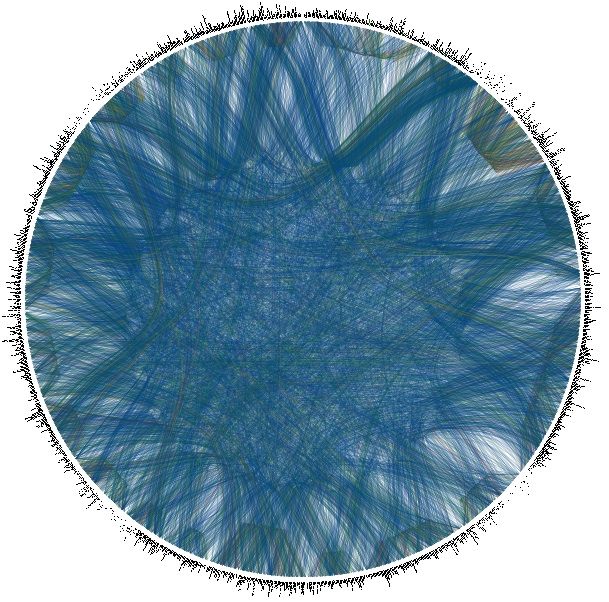
\includegraphics[width=0.48\textwidth]{img/completeNetworkLabels.jpg}
    \caption{Full network of all 1,288 concepts in CLiCs (outer circle) together with their connections. The strength of the connections is marked in different colors, with very strong links represented in red}
    \label{fig:clics_full}
\end{figure}
\subsection{Interactive functionalities}


% Force-directed graph; move nodes to desired position

The visualization features various interactive functionalities that are designed to enhance the exploration of the CLiCs data on the level of communities. The main component is a flexible force-directed graph layout that displays the concepts as nodes and the cross-linguistic polysemies as edges (see Figure \ref{EarthLand}). The strength of the force in the edges of the graph is dependent on the number of language families that can be attested to have lexical associations for the respective concepts that are linked through the edge. We decided to have separate graphs for all communities, which the user can select from a drop-down menu. As described above, the communities have been automatically generated from the whole network of concepts and links with the help of the Infomap algorithm for community detection \cite{Rosvall2008}. 

\begin{figure}[htbp]
\begin{center}
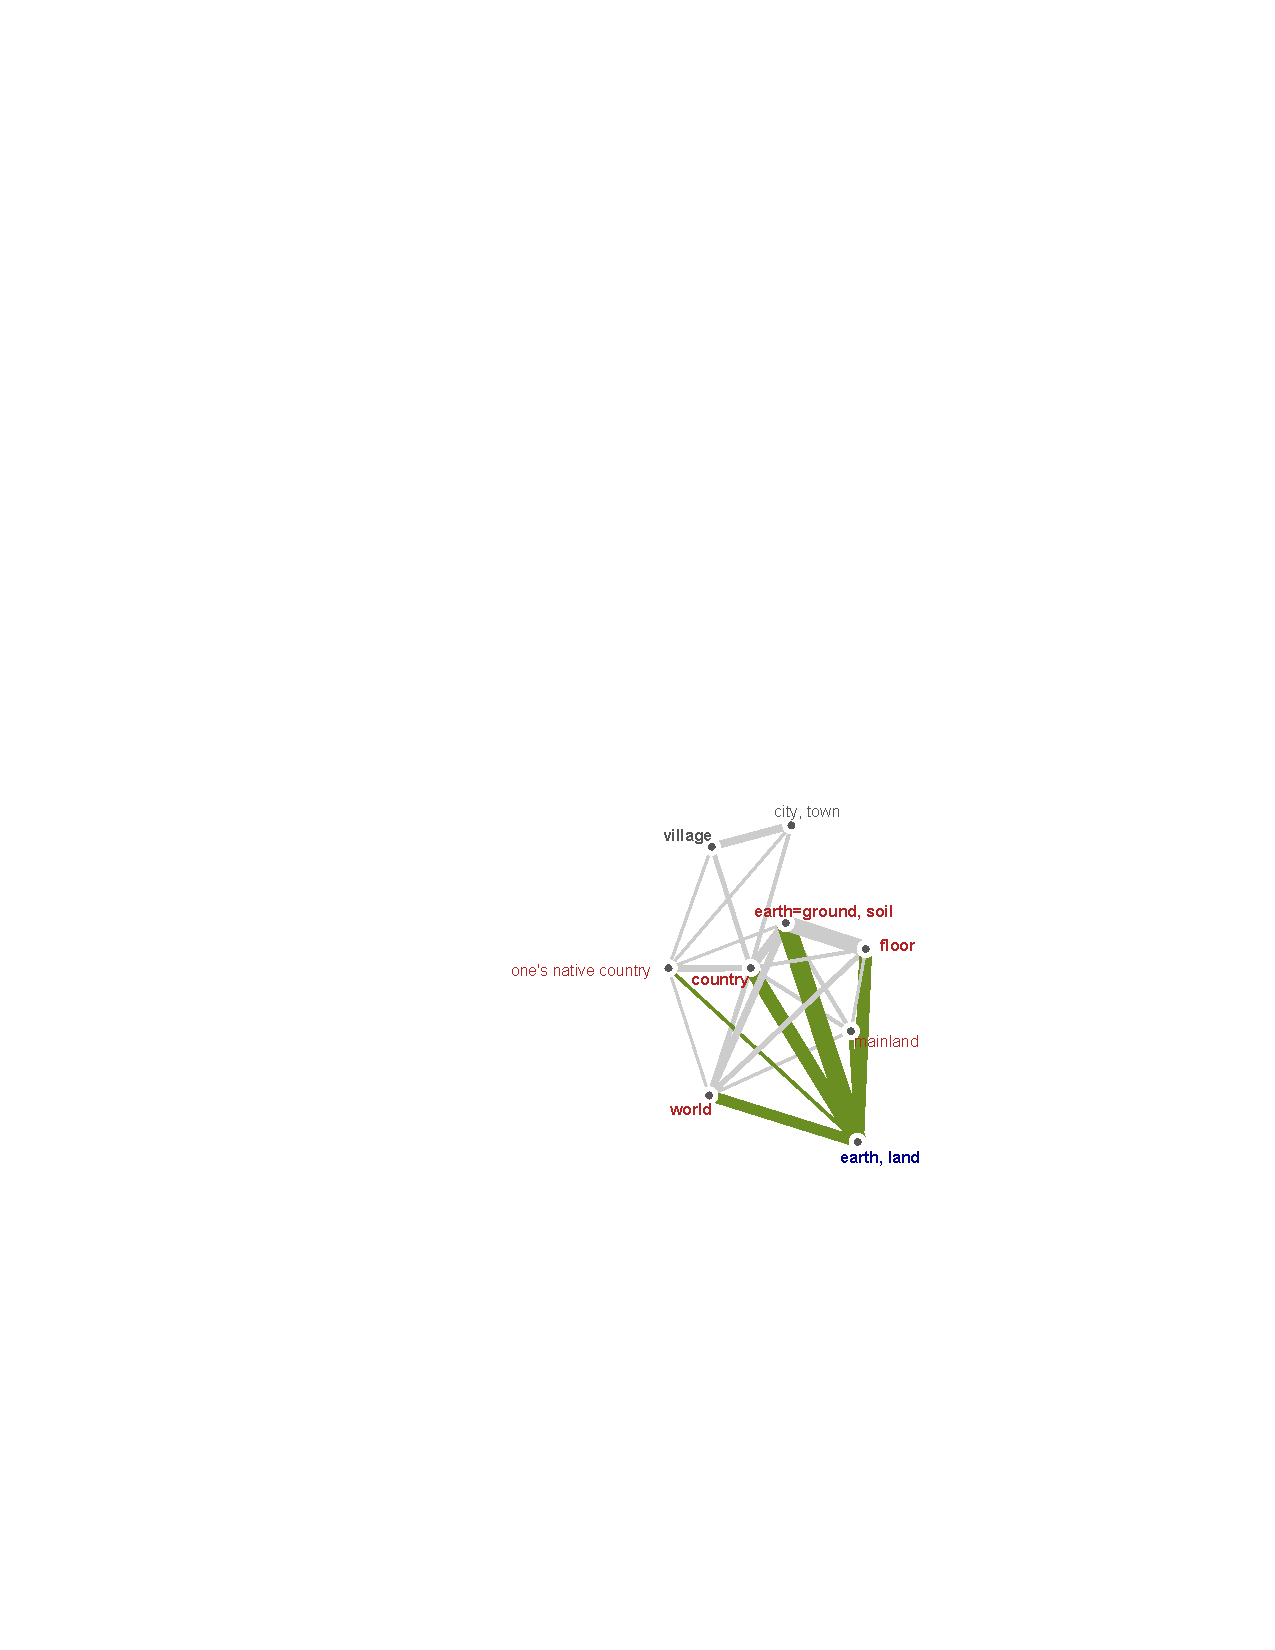
\includegraphics[width=0.48\textwidth]{img/earthland.pdf}
\caption{Force-directed graph with mouse-over functionalities highlighting all connected concepts}
\label{EarthLand}
\end{center}
\end{figure}

The force-directed graph layout ensures that all concepts are neatly arranged according to their similarity as defined by the number of cross-linguistic colexifications. As a result, concepts that are highly connected are located close to each other.  To make it easier for users to explore the network that is depicted in the graph, concepts can be dragged to different positions where there is less overlap. The dragging behavior of a concept  is activated when mousing over the respective node in the graph (when the cursor symbol turns into a crosshair).

\begin{figure*}[htbp]
\begin{center}
\includegraphics[width=\textwidth]{img/MoneySilverAreasNEU.pdf}
\caption{Force-directed graph with mouse-over functionalities showing one community in CLiCs (community 27: gold) together with a subset of the instances of a particular colexification pattern (left). The entries have different background colors depending on their location in the world map (cf. Figure \ref{World map})}
\label{MoneySilver}
\end{center}
\end{figure*}



% mouse-over: coloring edges, show linked languages

As mentioned above, the edges of the graph represent the number of cases of cross-linguistic colexifications for the linked concepts. For a more detailed view on which languages contribute to the strength of the connections, the user can mouse over the links in the graph to see a list of  languages featuring polysemous words for the respective link (Figure \ref{MoneySilver}). The list includes additional information on the languages such as their ISO 639-3 language code and family. Furthermore, each entry in the list provides a hyperlink to the original source from where the information is taken.  

% Color coding: families and geolocations

Each language in the list is attributed a different background color depending on its language family or location in order to allow for an at-a-glance overview of all languages in the list. The user can choose from a drop-down menu whether to include the genealogical or areal information as the background color. For the genealogical information, all language families are attributed a different color value. Languages belonging to the same language families are therefore given the same background color. Moreover, the list is sorted according to language families. In this way, the user can immediately see how many languages of  a given family contribute to the overall strength for the connection at hand. 

As to the areal information, the world map is provided with a color gradient as shown in Figure \ref{World map}. To this end, each position in the world map is attributed a color value using the L*a*b* color space. The color hue thereby indicates the position on the map in terms of the longitude (specifying the east-west position) whereas the lightness of the color represents the position in terms of the latitude information (specifying the north-south position).\footnote{See \newcite{MayerLanguageExplorer} for a different approach of a linguistically informed color gradient of the world map.}
The mapping from geolocation to color values allows for an easier evaluation of areal patterns in the selected connection. In this regard, users can directly detect whether a certain cross-linguistic polysemy is restricted to a certain region of the world or constitutes a more widespread colexification pattern (see the case study in Section \ref{case study} below).

\begin{figure}[htbp]
\begin{center}
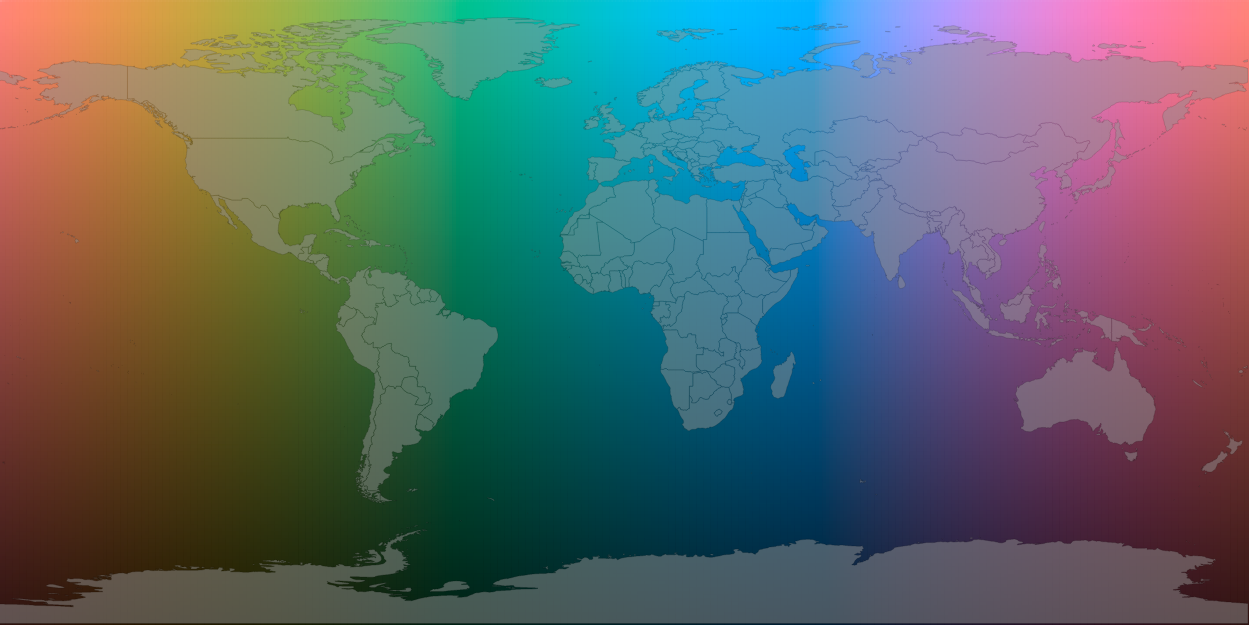
\includegraphics[width=0.48\textwidth]{img/ColorScaleWorld.png}
\caption{World map with color gradient}
\label{World map}
\end{center}
\end{figure}


% show only edges with a minimum number of links

In addition to the interactive functionalities described above, the visualization also features a variety of further components that allow for an easier exploration of the database. The graph layout is equipped with panning and zooming functionality that enables the user to navigate through the network graph. Panning is enabled when the cursor changes into a hand symbol when mousing over a link of the graph. The whole graph can then be dragged to a new position. The zooming behavior is activated with the scroll wheel. 
When mousing over a concept (node) in the graph all connected links and concepts are highlighted
in order to provide a better overview of the connectivity of certain concepts (see Figure \ref{EarthLand}). The control panel of the visualization also includes a slider button that allows the user to show only those edges in the graph with a minimum number of cross-linguistic colexifications. 

% zooming and panning



\subsection{Implementation}
% description of D3 and the implementation

The visualization is implemented in JavaScript using the D3 library \cite{D3}.\footnote{\url{http://d3js.org}} The force-directed graph is  generated with the \texttt{force()} function from the \texttt{d3.layout} module. The layout implementation uses position Verlet integration for simple constraints \cite{Dwyer2009}.\footnote{See \url{https://github.com/mbostock/d3/wiki/Force-Layout} for a description of the implementation.} In order to ensure that the concept labels are located close to the concept nodes, a second force layout (with a static weight of $1$) for each concept link to the node is set up. 

The color values for the world map gradient scale are computed from the two-dimensional geographical coordinates that are given as an input. The latitude [-90;90] and longitude [-180;180] values are thereby normalized between [0;1] and serve as the input for the function \texttt{cl2pix}.\footnote{The code was adapted from the GNU C code by David Dalrymple (\url{http://davidad.net/colorviz/}, accessed on January 25th, 2014) and translated into JavaScript.}

\begin{verbatim}
function cl2pix(c,l){
   		var TAU = 6.2831853 
   		var L = l*0.61 + 0.09; 
   		var angle = TAU/6.0 - c*TAU;   
   		var r = l*0.311 + 0.125 
   		var a = Math.sin(angle)*r;
   		var b = Math.cos(angle)*r;
   		return [L,a,b];
 };
\end{verbatim}

The actual HTML color code is generated with the function \texttt{d3.lab} from the D3 library, which takes as input the three values for \texttt{[L,a,b]}. The main reason for choosing the L*a*b* color space is a smoother transition between different color hues without any visible boundaries. As can be seen in Figure \ref{lab vs hsv}, the color gradient in the L*a*b* color space exhibits a much smoother perceptual transition between the color hues on the x-axis. 
%\footnote{See \url{http://davidad.net/colorviz/} for the difference between using the L*a*b* and HSV color space in terms of transitions between different color hues.} 
For the coloring of the language families, the background colors are generated with the categorical scale functions of the \texttt{d3.scale} module. 

\begin{figure}[h]
    \centering
   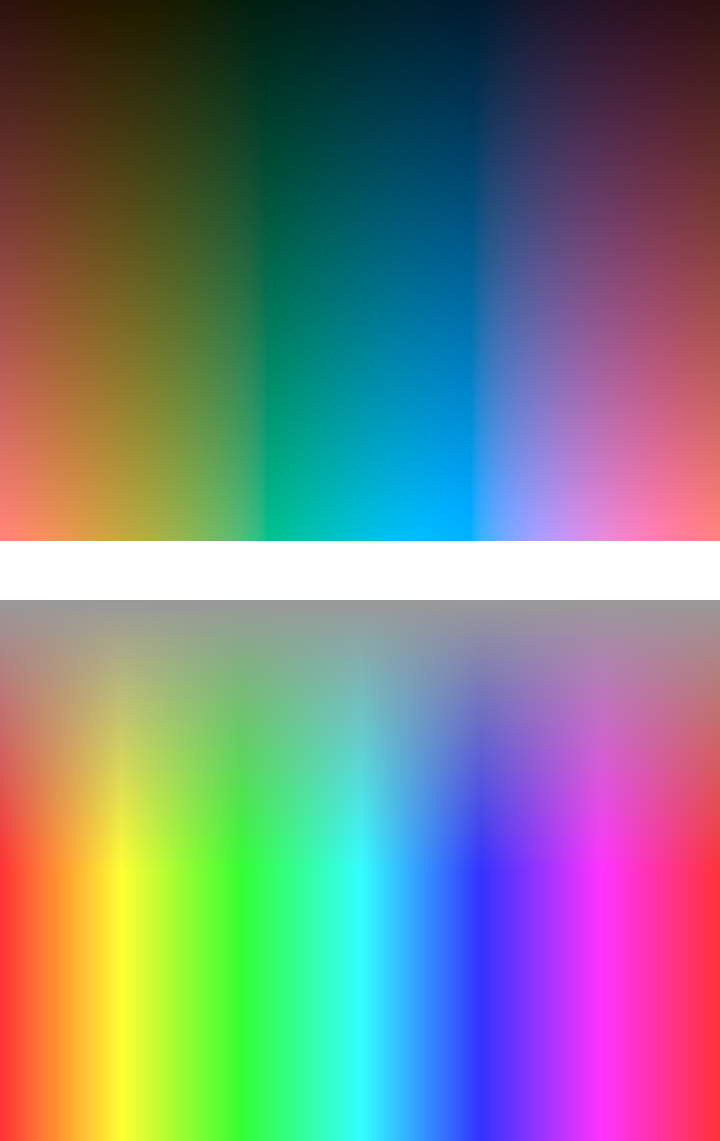
\includegraphics[width=0.48\textwidth]{img/Lab_HSV.png}
    \caption{Comparison between two-dimensional color gradients in the L*a*b* (top) and HSV (bottom) color space}
    \label{lab vs hsv}
\end{figure}


The  dragging and panning functionalities of the graph are implemented with the \texttt{drag()} function from the \texttt{d3.behavior} module and the SVG \texttt{transform} and \texttt{translate} attributes. 

\subsection{Case studies} \label{case study}

In order to illustrate the usefulness of the visualization for the purposes of exploring the database, consider the graph in Figure \ref{MoneySilver}. Among other things, it contains the connection between the concepts ``money'' and ``silver''. A subset of the languages and words contributing to this connection are shown on the left where the background color represents the location of the languages. For instance, French contributes to the cross-linguistic colexification because both concepts are realized by the same word (viz. \textit{argent}) in that language. When looking at the areal distribution of the languages, a clear pattern emerges at a glance (see Figure \ref{MoneySilverAreas} for the full list of languages showing this colexification pattern). Most of the languages contributing to the colexification are from two major regions: Caucasus (marked in blue) and South America (marked in green). However, as mentioned in Section \ref{caveats}, this distribution might be an artifact of the general bias for languages of the Caucasus and South America in the underlying databases. In any case, the visualization directly points the attention to this pattern. As the  aim of the visualization component is not to replace linguistic research but to guide it, such patterns have to be looked at in more detail by checking the actual data. 

\begin{figure}[htbp]
%\begin{center}
%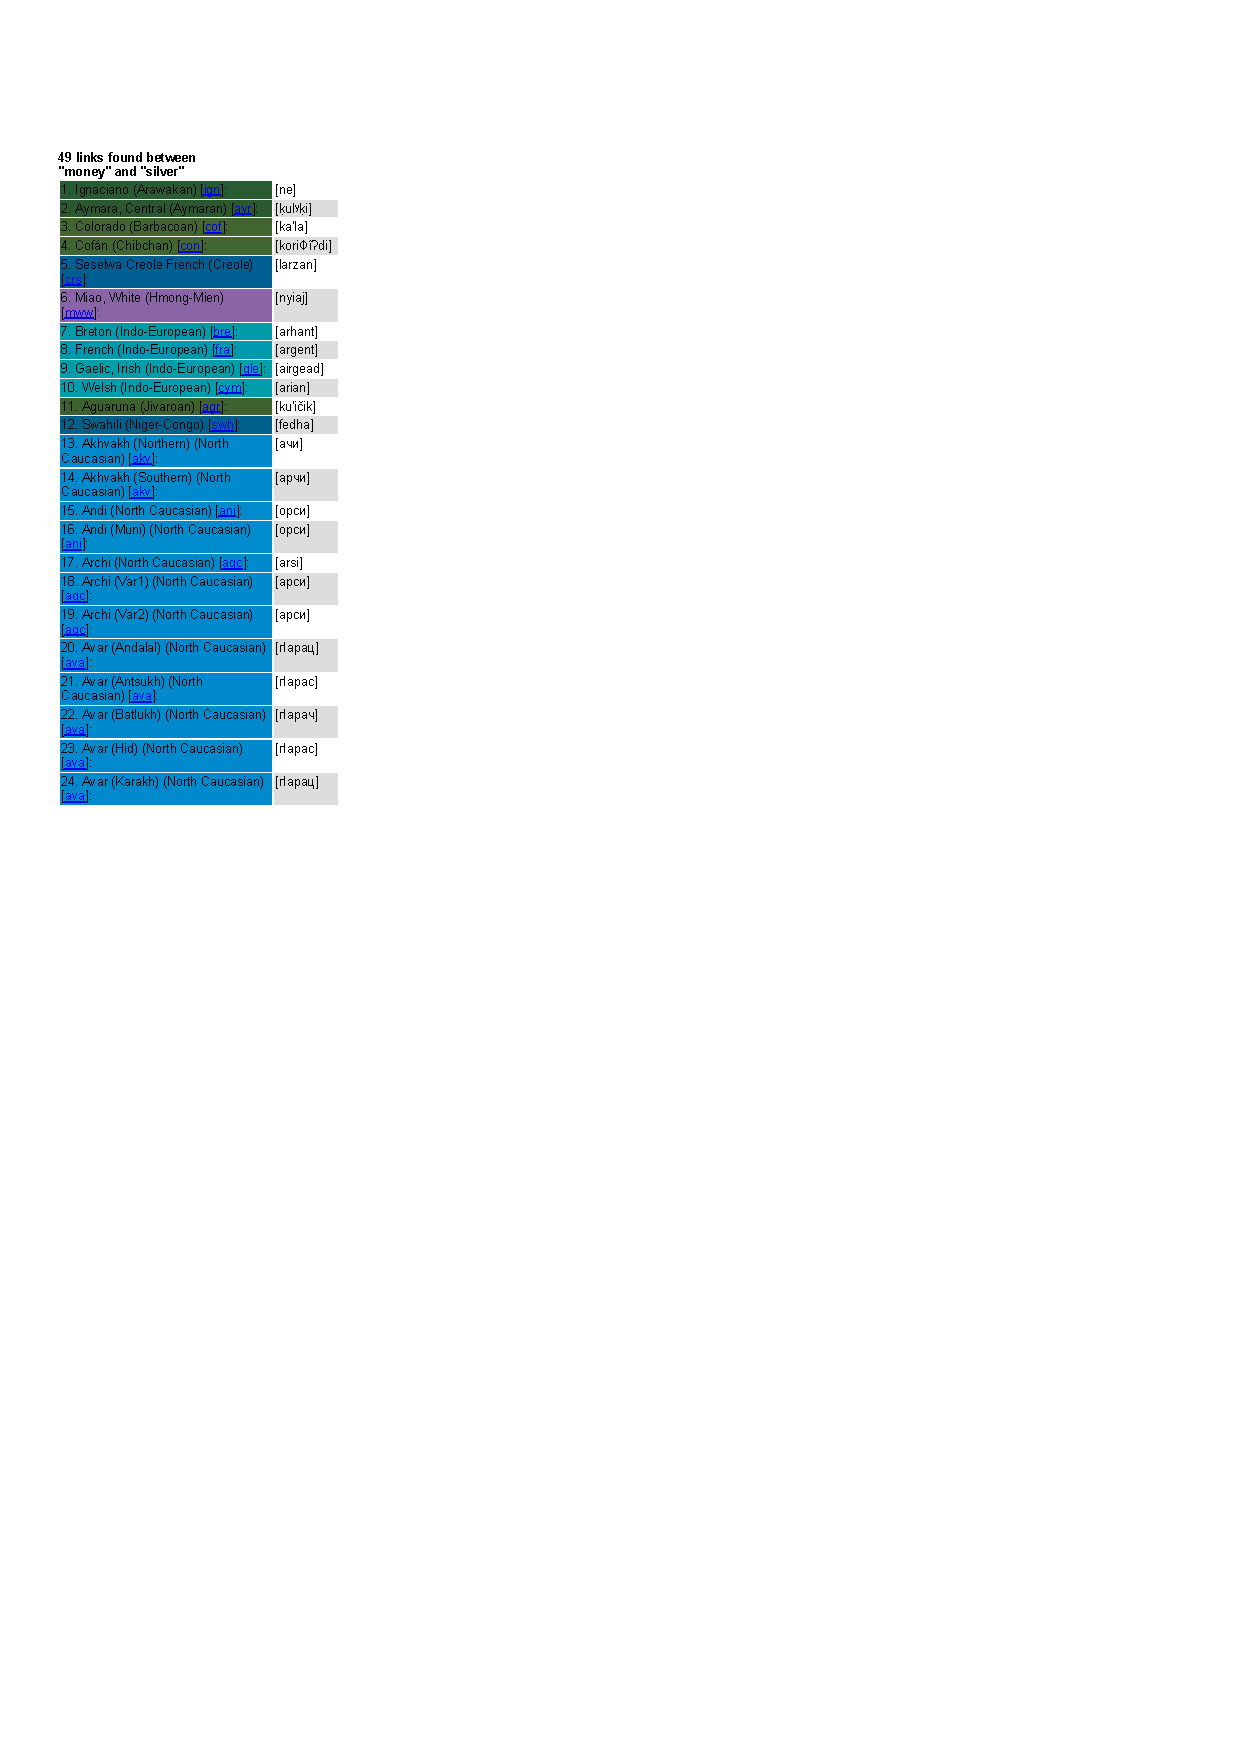
\includegraphics[width=0.238\textwidth]{img/moneysilverAreas1.pdf}
%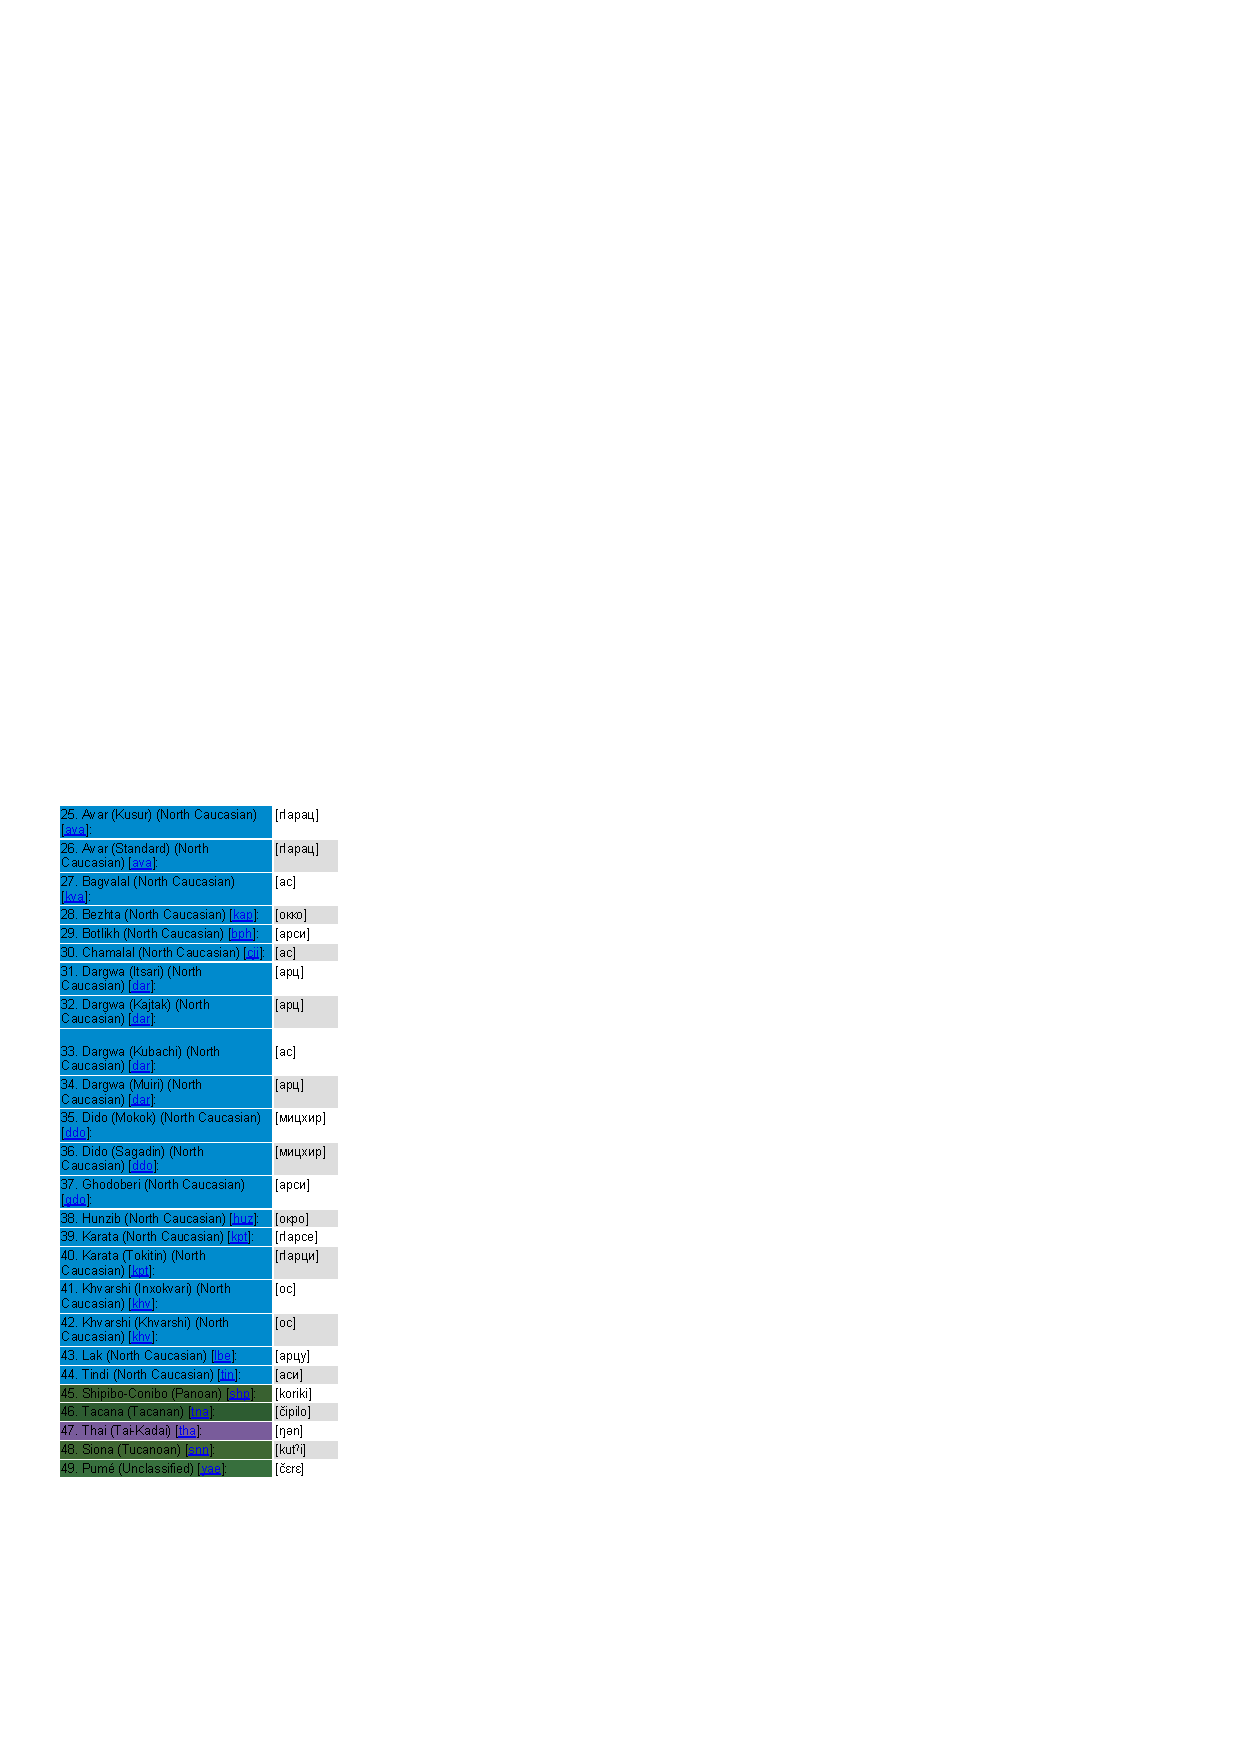
\includegraphics[width=0.238\textwidth]{img/moneysilverAreas2.pdf}
\hspace{-0.4cm}
\begin{tabular}[t]{ll}
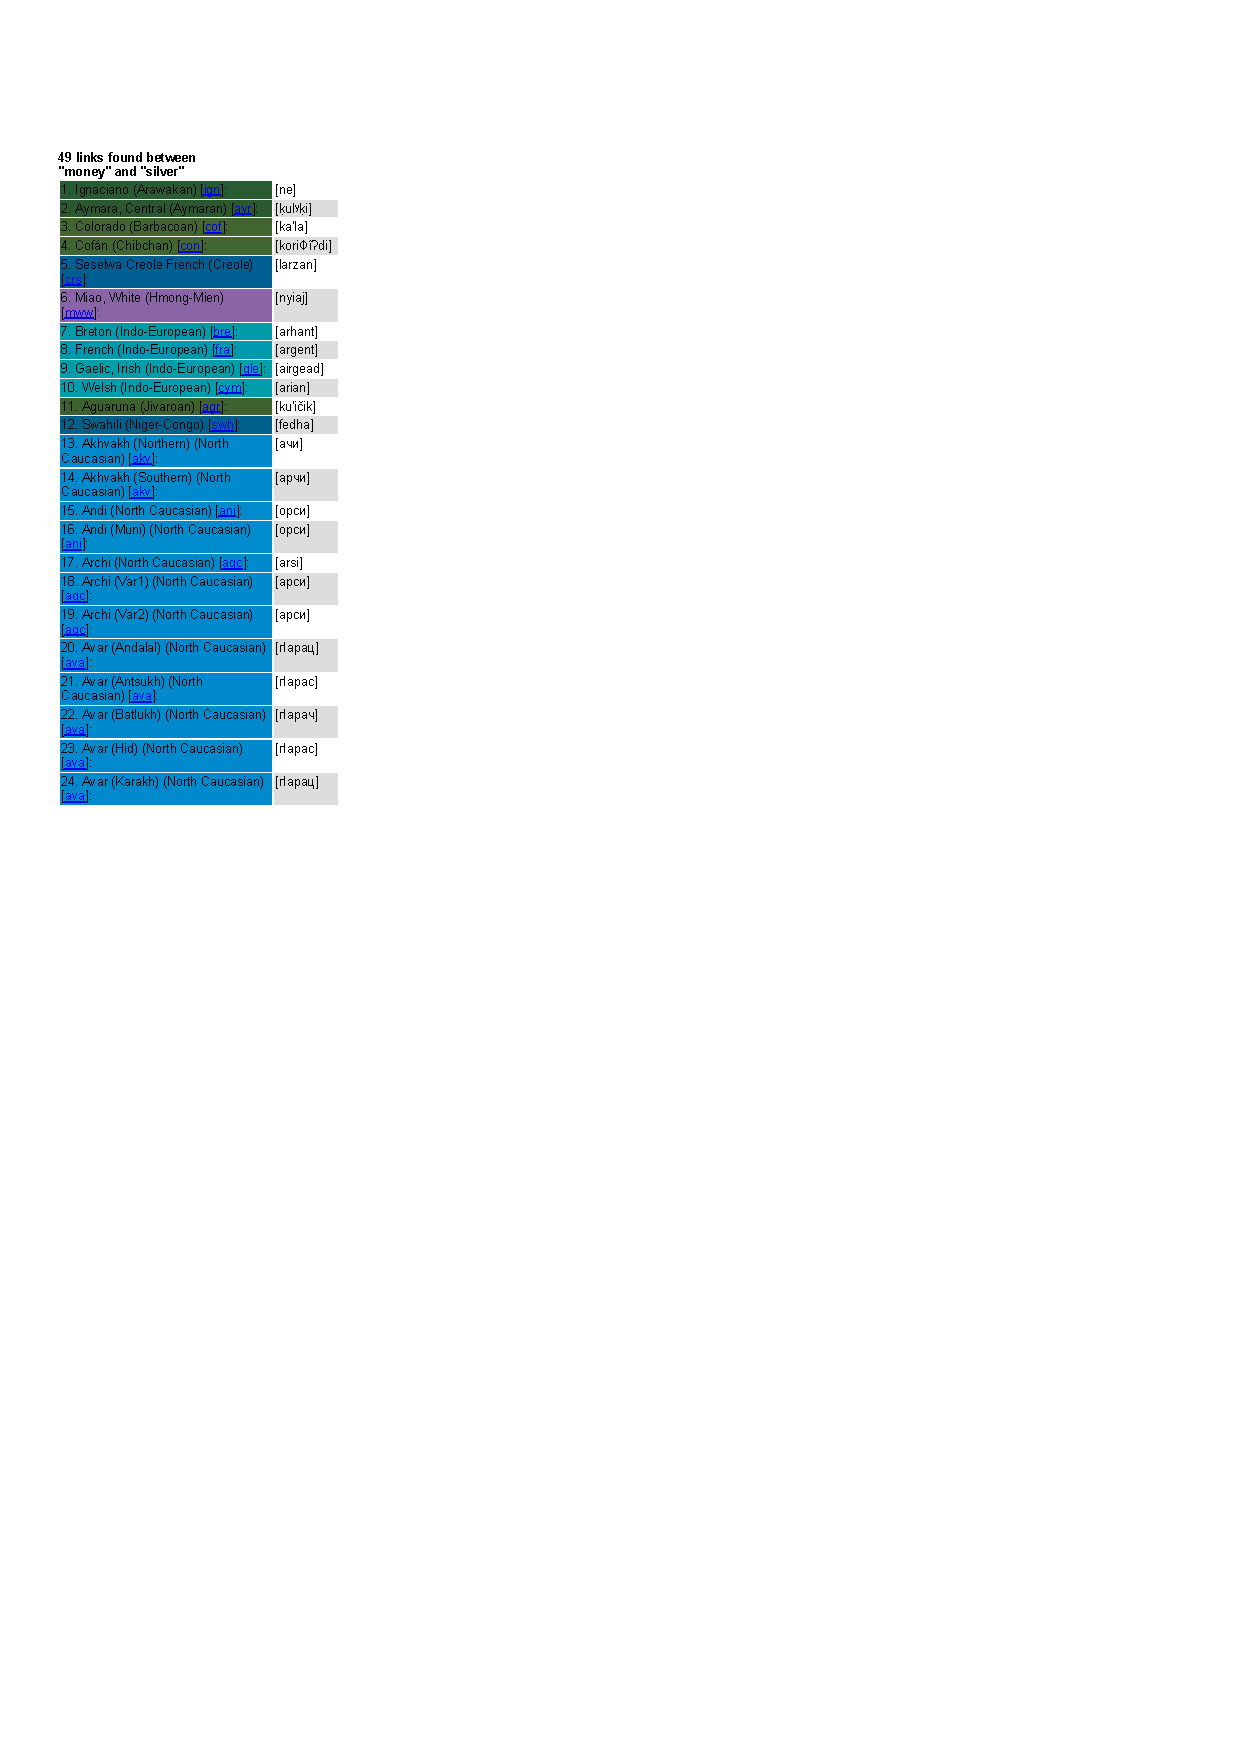
\includegraphics[width=0.238\textwidth]{img/moneysilverAreas1.pdf} &
\hspace{-0.2cm} \raisebox{2.8cm}{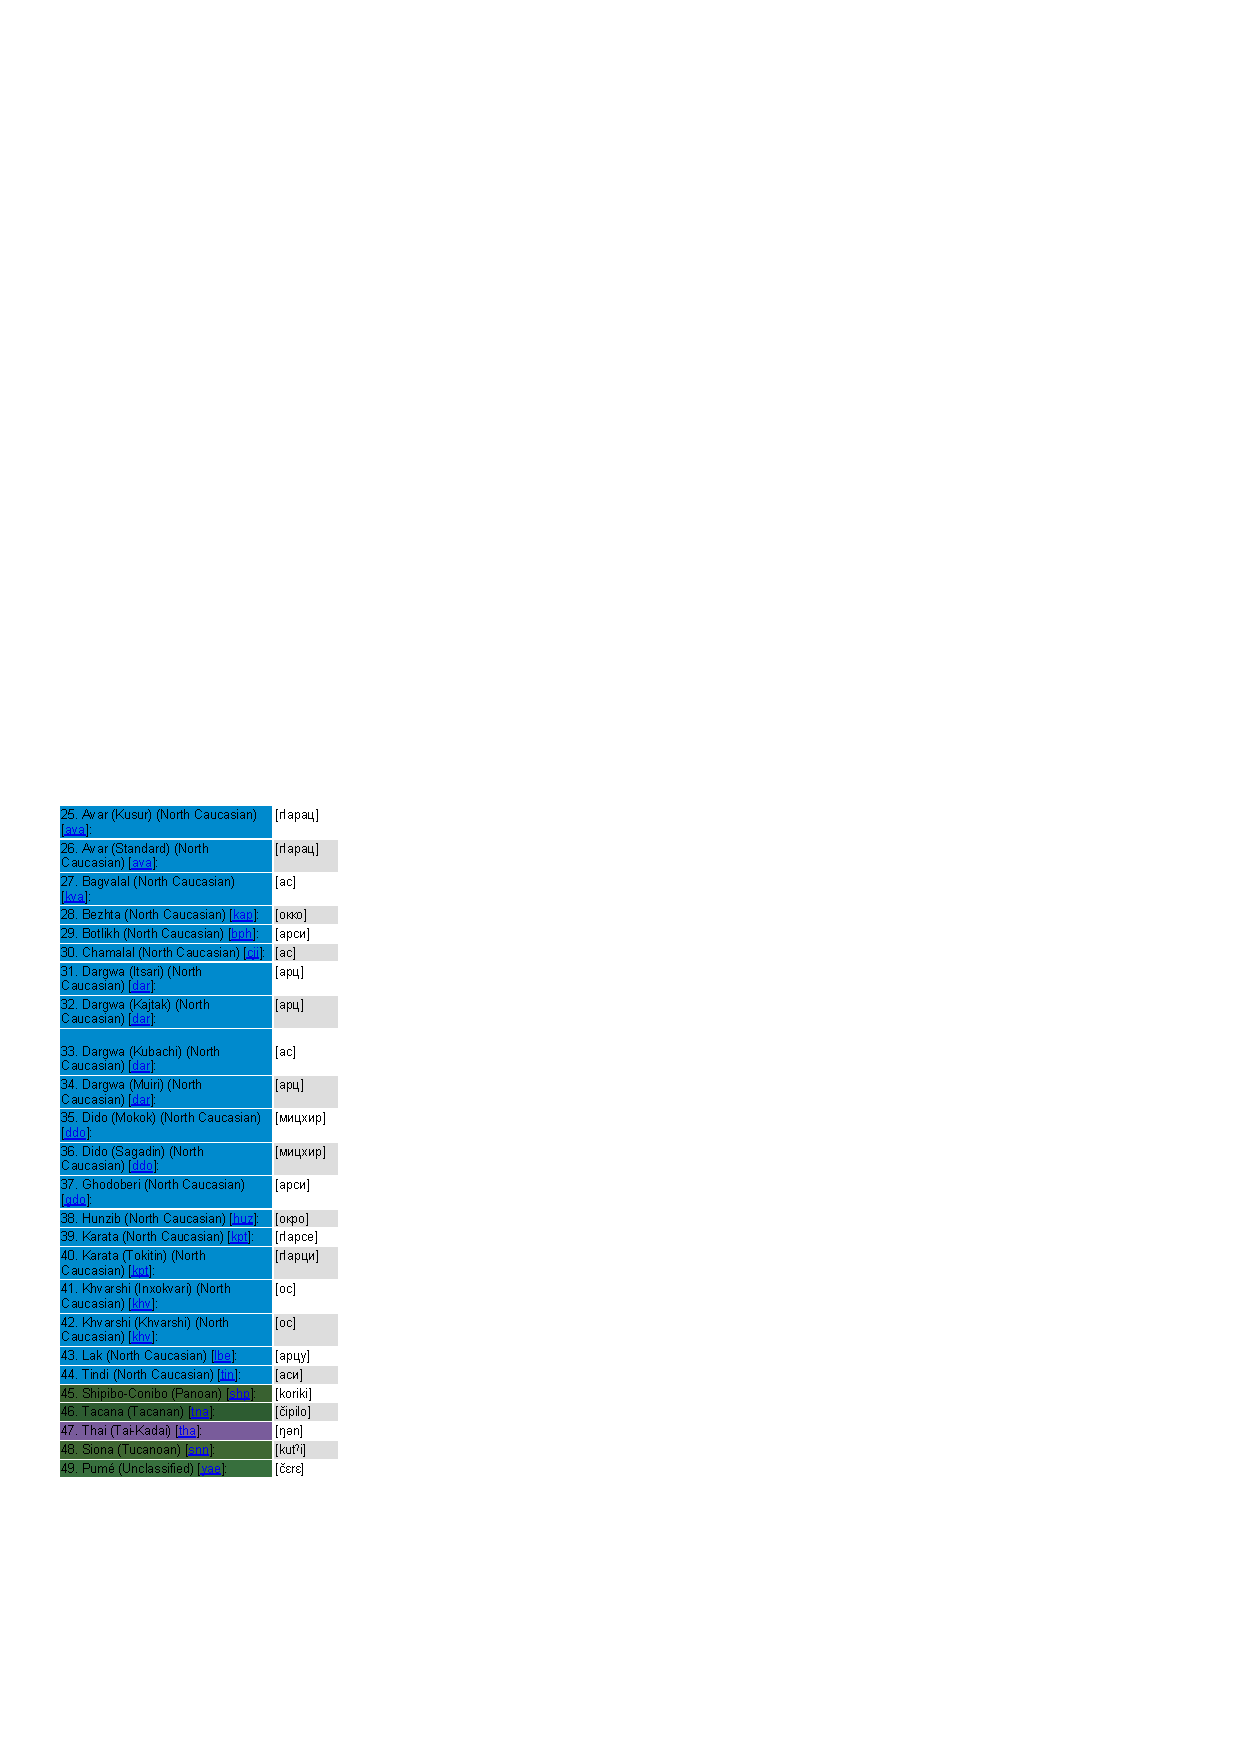
\includegraphics[width=0.238\textwidth]{img/moneysilverAreas2.pdf}}
\end{tabular}
\caption{Languages and words contributing to the connections of lexical associations for the concepts ``money'' and ``silver''}
\label{MoneySilverAreas}
%\end{center}
\end{figure}

\begin{figure*}[htbp]
\begin{center}
\includegraphics[width=\textwidth]{img/wheelfootAreal_new.pdf}
\caption{Force-directed graph with areal distribution for the concepts ``wheel'' and ``foot''}
\label{WheelFootAreas}
\end{center}
\end{figure*}


Another example deals with the colexification of the concepts ``wheel'' and ``foot''. In contrast to the case of ``money'' and ``silver'' above, these concepts at first glance may not immediately suggest a close association. Yet such cases do exits as the link in Figure \ref{WheelFootAreas} reveals. The connection links two bigger communities of nodes, including spherical objects on the one hand and parts of the lower body on the other. The list of languages for the connection ``wheel'' and ``foot'' in Figure \ref{WheelFootAreas} clearly shows that the association is restricted to languages of South America. 
This geographical restriction may reflect semantic borrowing among South American languages, but since the distribution within South America is rather erratic, independent innovation is also a possibility. At any rate, the color coding in the visualization immediately draws the researcher's attention to the potentially interesting geographical patterning.
%Even though the languages cover a range of different families, the areal distribution is clearly confined to a certain area. This might lead to the conclusion that the associations result from loan translations of the concept through language contact (the lexical entries show that they are most likely not cognates and that the association is thus due to loan words for both concepts). However, such a preliminary hypothesis has to be confirmed by looking at the actual data. 





\section{Conclusions and future work}

The size and complexity of today's language resources call for a data preparation pipeline that enables researchers to find meaningful patterns among the multitude of different factors that can be taken into consideration. In our view, such a data preparation pipeline necessarily consists of two major parts, both of which are illustrated in the present paper. On the one hand, methods and techniques from data mining or computational linguistics help to detect basic trend or groups of similar objects in the search space. On the other hand, the resulting groups or trends are mapped to visual variables in order to make interesting observations readily accessible to human perception. 

The CLiCs database contains a wealth of information about colexification patterns in the languages of the world. Manually inspecting the large amount of connections in the database, however, is a laborious and time-consuming task that allows for a detailed exploration of individual links but does not capture overall trends in the data. This paper presents an attempt to combine the advantages of human inspection with the strength of a computational approach \cite{Keim2008}. 

The CLiCs visualization features an automatic preprocessing of the colexification links into so-called communities of the graph, groups of highly connected nodes that reveal a meaningful overall trend in the worldwide patterns of lexical associations. The communities are then graphically represented in a force-directed graph that shows all connections within the various concepts that are included. Interactive components in the visualization allow for a more detailed view of associations on the level of the languages that contribute to the colexification. 
Mapping the genealogical and areal information on individual languages to colors enables an at-a-glance evaluation of potentially interesting trends in individual colexifications (see the case studies in Section \ref{case study}). 
In this way, users can get an overview of the general trends in the data and at the same time have the opportunity to directly inspect the lexical associations. 

In future work, we plan to enhance the visualization tool with further interactive components that allow for a better overview of the complete network of colexifications (shown in Figure \ref{fig:clics_full}) and facilitate the detection of genealogical or areal trends in the database. The idea is to integrate a sunburst visualization \cite{Sunburst}  for the genealogical information in order to enable a better overview of the language families that are involved in a given colexification pattern.\footnote{See \cite{MayerLanguageExplorer} for an example of using sunburst displays to represent the hierarchical structure of language families.} In addition, we intend to equip the user interface with further interactive components that allow users to explore the database from different perspectives (e.g., compare individual languages in terms of shared lexical associations). All components will be made publicly available online for the (linguistic) research community. 


\bibliographystyle{lrec2014}
\bibliography{clicsvis}

\end{document}

